\documentclass[10pt,twocolumn,letterpaper]{article}

\usepackage{cvpr}
\usepackage{times}
\usepackage{epsfig}
\usepackage{graphicx}
\usepackage{amsmath}
\usepackage{amssymb}
\usepackage[utf8]{inputenc}
\usepackage{cite}
\usepackage{listings}
\usepackage[portuguese,ruled,lined]{algorithm2e}
\usepackage{spverbatim}

%\usepackage[breaklinks=true,bookmarks=false]{hyperref}

\cvprfinalcopy

\def\cvprPaperID{****}
%\def\httilde{\mbox{\tt\raisebox{-.5ex}{\symbol{126}}}}


\setcounter{page}{1}
\begin{document}

\title{\Huge Utilização do algoritmo PSO para ajuste dos pesos em redes RBF}

\author{Daniel Vilas-Boas\\
\footnotesize Departamento de Estatística e Informática\\
\footnotesize Universidade Federal Rural de Pernambuco\\
{\tt\small daanielvb@gmail.com}
\and
Leonardo Figueiroa\\
\footnotesize Departamento de Estatística e Informática\\
\footnotesize Universidade Federal Rural de Pernambuco\\
{\tt\small leonardofigueiroa@live.com}
\and
Rodrigo Cunha\\
\footnotesize Departamento de Estatística e Informática\\
\footnotesize Universidade Federal Rural de Pernambuco\\
{\tt\small r-cunha@outlook.com}
}

\maketitle
%\thispagestyle{empty}

\begin{abstract}
O uso de redes neurais de base radial ou RBFs vem sendo bastante utilizadas para classificação de padrões por apresentar diversas vantagens sobre outras redes (como a MLP), apresentando um treinamento mais eficiente e melhor grau de separabilidade. Este trabalho envolveu o desenvolvimento de uma RBF em conjunto com o algoritmo de otimização por enxame de partículas ou PSO. A rede neural foi desenvolvida de forma que seus pesos de saída fossem ajustados pelo PSO visando obter os melhores pesos na camada de saída e consequentemente menor taxa de erro e melhor classificação das características de entrada.\\
\begin{center}
\textbf{\textit{Keywords --- RBF; PSO; redes neurais; classificação de padrões}}\\
\end{center}
\end{abstract}


\section{Introdução}
As redes denominadas \textit{funções de base radial}, convencionalmente conhecidas como \textit{RBF (radial basis function)}, são usadas em variados tipos de problemas tais como aproximação de funções e classificação de padrões. Ela pertence a arquitetura \textbf{feedforward} de camas múltiplas, cujo treinamento é efetivado de forma supervisionada. Sua estrutura é composta tipicamente por apenas uma camada intermediária, na qual as funções de ativação são do tipo \textit{gaussiana}. O fluxo de informações tem início na camada de entrada, passando então pela respectiva camada intermediária, e finalizando na camada neural de saída com neurônios com funções de ativação linear~\cite{livroAula}.\\ 

O \textit{PSO (Particle Swarm Optimization)} é um algoritmo de otimização por enxame de partículas. Tem uma abordagem \textbf{estocástica}, baseada em população que simula o processo comportamental de interação entre os indivíduos de um grupo. Sua teoria é baseada em comportamento de atividades de grupos de animais como pássaros e peixes, que realizam tarefas de otimização na execução de atividades como a busca por alimentos. O \textit{PSO} se inicia com um enxame de partículas com posições aleatórias. Cada partícula é dita ser uma possível solução para o problema investigado, sendo atribuído a cada indivíduo (partícula) um valor que está relacionado a adequação da partícula com a solução do problema (denominada \textbf{fitness}), e, também, uma variável velocidade que representa a direção do movimento da partícula. Com o passar do tempo, as partículas vão ajustando suas velocidades em relação a seu melhor \textbf{fitness}, encontrada pela própria partícula, e também pela melhor solução do grupo de partículas.\\ Elas continuam realizando este processo até que encontrem uma solução ótima. O valor \textbf{fitness} é definido pela natureza do problema de otimização e é computada por uma função objetivo que avalia um vetor solução. \\

Neste papel são discutidos a implementação da rede neural \textit{RBF} em conjunto com o algoritmo de otimização \textit{PSO}, os experimentos realizados após a implementação, e os resultados encontrados após os experimentos realizados.


%-------------------------------------------------------------------------
\subsection{Procedimentos}
Nesta seção serão discutidos os procedimentos realizados pela rede neural e pelo algoritmo de otimização. Os procedimentos são outros algoritmos conhecidos na literatura de \textbf{inteligência artificial} e \textbf{redes neurais artificiais} (como o \textit{kMeans} e a \textit{RBF}). Serão brevemente discutidos como funcionam e o seu papel na implementação do projeto. No \textbf{apêndice} pode ser encontrado o código-fonte do projeto para eventual consulta. O código-fonte foram escritos em linguagem \textit{Java}.

\subsection{kMeans}

Pellentesque mauris sem, blandit tempor scelerisque nec, dictum sed lorem. Proin in libero a elit bibendum volutpat vitae a ligula. Aliquam sagittis ligula quis auctor sollicitudin. Sed eget blandit elit, ac sagittis dolor. Vestibulum in eros a nibh venenatis fermentum sit amet nec nibh. Suspendisse hendrerit cursus eros, eu ornare nisi placerat id. Phasellus venenatis eget velit eu consectetur. Sed elementum magna a venenatis cursus. Vivamus gravida viverra neque, et laoreet ipsum. Mauris pellentesque libero quis tincidunt ullamcorper. Donec egestas faucibus blandit. Morbi bibendum nibh eget dignissim congue. Sed maximus quis dolor quis congue. In hac habitasse platea dictumst.

\subsection{Radial Basis Function --- RBF}
Pellentesque mauris sem, blandit tempor scelerisque nec, dictum sed lorem. Proin in libero a elit bibendum volutpat vitae a ligula. Aliquam sagittis ligula quis auctor sollicitudin. Sed eget blandit elit, ac sagittis dolor. Vestibulum in eros a nibh venenatis fermentum sit amet nec nibh. Suspendisse hendrerit cursus eros, eu ornare nisi placerat id. Phasellus venenatis eget velit eu consectetur. Sed elementum magna a venenatis cursus. Vivamus gravida viverra neque, et laoreet ipsum. Mauris pellentesque libero quis tincidunt ullamcorper. Donec egestas faucibus blandit. Morbi bibendum nibh eget dignissim congue. Sed maximus quis dolor quis congue. In hac habitasse platea dictumst.
\begin{figure}[h]
\begin{center}
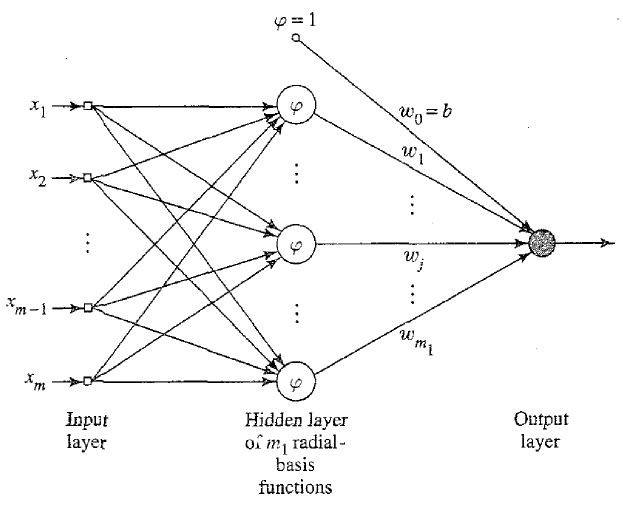
\includegraphics[scale=0.3]{foto1.jpg}
\caption{\textit{Estrutura teórica da RBF}}
\end{center}
\end{figure}
Pellentesque mauris sem, blandit tempor scelerisque nec, dictum sed lorem. Proin in libero a elit bibendum volutpat vitae a ligula. Aliquam sagittis ligula quis auctor sollicitudin. Sed eget blandit elit, ac sagittis dolor. Vestibulum in eros a nibh venenatis fermentum sit amet nec nibh. Suspendisse hendrerit cursus eros, eu ornare nisi placerat id. Phasellus venenatis eget velit eu consectetur. Sed elementum magna a venenatis cursus. Vivamus gravida viverra neque, et laoreet ipsum. Mauris pellentesque libero quis tincidunt ullamcorper. Donec egestas faucibus blandit. Morbi bibendum nibh eget dignissim congue. Sed maximus quis dolor quis congue. In hac habitasse platea dictumst.

\subsection{Particle Swarm Optimisation --- PSO}
Pellentesque mauris sem, blandit tempor scelerisque nec, dictum sed lorem. Proin in libero a elit bibendum volutpat vitae a ligula. Aliquam sagittis ligula quis auctor sollicitudin. Sed eget blandit elit, ac sagittis dolor. Vestibulum in eros a nibh venenatis fermentum sit amet nec nibh. Suspendisse hendrerit cursus eros, eu ornare nisi placerat id. \\

\begin{algorithm}[]
\Inicio{
\ParaCada {particula}{
inicialize a particula\;
}
\Repita{número de épocas ser atingido}{
\ParaCada{particula}{
calcule o valor do fitness\;
\Se {fitness for melhor que o fitness em pBest}{
guarde o valor como o novo pBest\;
}
}
Escolha a particula com melhor valor de fitness de todas as particulas como a gBest\;
\ParaCada {particula}{
calcule a velocidade de acordo com a equação (a)\;
atualize a posição de acordo com a equação (b)\;
}
}
}
\caption{Pseudo-código do PSO}
\end{algorithm}

Phasellus venenatis eget velit eu consectetur. Sed elementum magna a venenatis cursus. Vivamus gravida viverra neque, et laoreet ipsum. Mauris pellentesque libero quis tincidunt ullamcorper. Donec egestas faucibus blandit. Morbi bibendum nibh eget dignissim congue. Sed maximus quis dolor quis congue. In hac habitasse platea dictumst.

%-------------------------------------------------------------------------

\section{Experimentos}

\subsection{Variando o número de neurônios, épocas e partículas}
Pellentesque mauris sem, blandit tempor scelerisque nec, dictum sed lorem. Proin in libero a elit bibendum volutpat vitae a ligula. Aliquam sagittis ligula quis auctor sollicitudin. Sed eget blandit elit, ac sagittis dolor. Vestibulum in eros a nibh venenatis fermentum sit amet nec nibh. Suspendisse hendrerit cursus eros, eu ornare nisi placerat id. Phasellus venenatis eget velit eu consectetur. Sed elementum magna a venenatis cursus. Vivamus gravida viverra neque, et laoreet ipsum. Mauris pellentesque libero quis tincidunt ullamcorper. Donec egestas faucibus blandit. Morbi bibendum nibh eget dignissim congue. Sed maximus quis dolor quis congue. In hac habitasse platea dictumst.

Nullam pulvinar nunc nec interdum sodales. Cras elit erat, gravida id tortor eu, molestie volutpat felis. Duis quis ipsum sapien. Etiam nec porttitor est. Vestibulum neque leo, sagittis id interdum vitae, congue a mi. Vestibulum interdum ipsum id viverra egestas. Suspendisse iaculis turpis nibh, a viverra dolor tempor eget. Donec volutpat, sapien a auctor venenatis, justo enim gravida nisi, vitae laoreet ipsum ligula sit amet mauris. Proin rhoncus auctor lectus, in dignissim elit.

\subsection{Observações}
Nullam pulvinar nunc nec interdum sodales. Cras elit erat, gravida id tortor eu, molestie volutpat felis. Duis quis ipsum sapien. Etiam nec porttitor est. Vestibulum neque leo, sagittis id interdum vitae, congue a mi. Vestibulum interdum ipsum id viverra egestas.

\section{Conclusão}

Nullam pulvinar nunc nec interdum sodales. Cras elit erat, gravida id tortor eu, molestie volutpat felis. Duis quis ipsum sapien. Etiam nec porttitor est. Vestibulum neque leo, sagittis id interdum vitae, congue a mi. Vestibulum interdum ipsum id viverra egestas. Suspendisse iaculis turpis nibh, a viverra dolor tempor eget. Donec volutpat, sapien a auctor venenatis, justo enim gravida nisi, vitae laoreet ipsum ligula sit amet mauris. Proin rhoncus auctor lectus, in dignissim elit.

{\small
\bibliographystyle{ieee}
\bibliography{rna}
}

\newpage
\onecolumn
   
\section*{Apêndice}
Aqui encontram-se os códigos escritos durante a implementação do projeto.
\section*{Pacote kmeans --- AuxiliaryFunctions.java}

\begin{spverbatim}
package kmeans;

public class AuxiliaryFunctions {
	
	/*
	 * Euclidean distance in 4 dimensions between Ponto
	 */
	public static double calculateEuclideanDistance4Dimensions(Ponto v, Ponto w){
		double result = Math.sqrt(Math.pow((w.getX() - v.getX()),2) + Math.pow((w.getY() - v.getY()),2) +
						Math.pow((w.getZ() - v.getZ()),2) + Math.pow((w.getW() - v.getW()),2) );
		return result;
	}
	
	/*
	 * Eucliadean distance in 4 dimensions between Ponto and Cluster
	 */
	public static double calculateEuclideanDistance4Dimensions(Ponto v, Cluster c){
		double result = Math.sqrt(Math.pow((c.getCenter().getX() - v.getX()),2) + Math.pow((c.getCenter().getY() - v.getY()),2) +
						Math.pow((c.getCenter().getZ() - v.getZ()),2) + Math.pow((c.getCenter().getW() - v.getW()),2) );
		return result;
	}
	
	/*
	 * Calculates RBF weights between input and intermediate layers
	 */
	public static double calculateRBFWeights(Ponto centro,Ponto p,double varianca ){
		return Math.exp(-Math.pow(calculateEuclideanDistance4Dimensions(centro,p),2)/2* (Math.pow(varianca,2)));
	}
}

\end{spverbatim}

\newpage
\section*{Pacote kmeans --- Cluster.java}

\begin{spverbatim}
package kmeans;

import java.util.ArrayList;

public class Cluster {
	private Ponto center;
	private ArrayList<Ponto> contains;
	private Double variance;
	
	//Constructor
	
	

	public Cluster(ArrayList <Ponto> ar,int size){
		int index = (int)(Math.random()*size);
		Ponto pt = ar.get(index);
		
		this.center = pt;
		this.contains = new ArrayList<Ponto>();
		
	}
	
	//Adds Ponto to itself
	
	public void addPonto(Ponto p){
		this.contains.add(p);
	}
	
	//Recalculate new center based on its points mean 
	
	public void CalculateNewCenter(){
		int size = this.contains.size();
		if(size == 0){
			//System.out.println("Empty Cluster");
		}
		else{
		double sumX = 0;
		double sumY = 0;
		double sumZ = 0;
		double sumW = 0;
		for (int i = 0; i < size ; i++){
			sumX += this.contains.get(i).getX();
			sumY += this.contains.get(i).getY();
			sumZ += this.contains.get(i).getZ();
			sumW += this.contains.get(i).getW();
		}
		this.center.setX(sumX/size);
		this.center.setY(sumY/size);
		this.center.setZ(sumZ/size);
		this.center.setW(sumW/size);
	}
	}
	
	//Verify if the Cluster has changed position
	
	public boolean hasChangedPosition(){
		double oldx = this.center.getX();
		double oldy = this.center.getY();
		double oldz = this.center.getZ();
		double oldw = this.center.getW();
		this.CalculateNewCenter();
		if(this.getCenter().getX() == oldx && this.getCenter().getY() == oldy &&
			this.getCenter().getZ() == oldz && this.getCenter().getW() == oldw){
			return false;
		}
		return true;
	}
	
	public void calculateVariance(){
		if(this.getContains().size() == 0){
			this.variance = 0.0;
		}
		else{
			Double sum = 0.0 ;
			for (int i = 0; i < this.getContains().size(); i++) {
				sum += AuxiliaryFunctions.calculateEuclideanDistance4Dimensions(this.getCenter(), this.getContains().get(i));
			}
			this.variance = sum/this.getContains().size();
		}
	}
	// Getters & setters
	
	public Ponto getCenter() {
		return center;
	}
	public void setCenter(Ponto center) {
		this.center = center;
	}
	public ArrayList<Ponto> getContains() {
		return contains;
	}
	public void setContains(ArrayList<Ponto> contains) {
		this.contains = contains;
	}
	
	public Double getVariance() {
		return variance;
	}

	public void setVariance(Double variance) {
		this.variance = variance;
	}
	
}

\end{spverbatim}
\end{document}
